
% DOCUMENT


\section{Metodología de trabajo}
\subsection {Metodología a seguir}
\par Es importante escoger una buena metodología de trabajo para poder desarrollar aplicaciones, ya que nos proporcionará todas las herramientas y procedimientos que se necesitan para conseguir un buen resultado y reducir el riesgo.
\par Las metodologías que se han escogido para este proyecto son: Craig Larman y Métrica V3. Es necesario utilizar Métrica V3 para poder definir correctamente todo el proyecto software, ya que hay algunos aspectos que no están contemplados en la metodología de Craig Larman, y viceversa.
\par La metodología Craig Larman parte de uno de los modelos de proceso descritos en el Unified Process. Con el objetivo realizar el trabajo de una manera más eficiente, el UP aplica técnicas iterativas, incrementales y dirigidas por casos de uso. El método Craig Larman se compone de tres fases:
\begin{enumerate}[1.]
\item \textbf{Planificación y especificación de requisitos:} esta etapa consiste en definir todos los requisitos necesarios en el sistema, así como los casos de uso. Además, se realizará un borrador del modelo conceptual del sistema.
\item \textbf{Construcción:} esta etapa es iterativa, debido a que de esta manera se consigue refinar el proyecto en cada una de las iteraciones. En cada una de ellas van surgiendo cambios que pueden llegar a afectar a próximas versiones, y por lo tanto, no se desperdician recursos. Para cada iteración se realiza un análisis, diseño, implementación y pruebas de un número reducido de casos de uso.
\begin{figure}[H]
\begin{center}
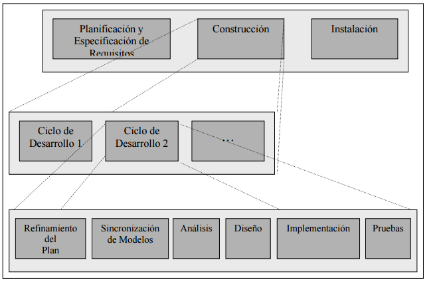
\includegraphics[width=0.6\textwidth]{./img/Metodologia.png}
\end{center}
\caption{Fase de construcción}
\label{tab:horasTotales}
\end{figure}

\item \textbf{Instalación:} una vez se alcanza la versión deseada por el cliente, se procede a la entrega del software.
\end{enumerate}
\par Métrica V3 ha sido desarrollada en España por el Ministerio de Administraciones Públicas, debido a la necesidad de estandarizar una metodología para el desarrollo de proyectos software. Principalmente, está dirigida a las empresas públicas, aunque también es posible aplicarlo en las empresas privadas.
\par Para el desarrollo del proyecto, se ha utilizará los siguientes apartados ya que no están tan detallados en la metodología Craig Larman:
\begin{enumerate}[1.]
\item Requisitos y estudio de la viabilidad del sistema
\item Plan de gestión de la calidad
\item Plan de gestión de la configuración
\item Organización y planificación
\end{enumerate}
